\documentclass[conference]{IEEEtran}
\IEEEoverridecommandlockouts
% The preceding line is only needed to identify funding in the first footnote. If that is unneeded, please comment it out.
%\usepackage{cite}
\usepackage[parfill]{parskip}
\usepackage{hyperref}
\usepackage{extarrows}
\usepackage{centernot}
\usepackage{mathtools}
\usepackage{braket}
\usepackage{mathpartir}
\usepackage{listings}
\usepackage{zi4}
\usepackage{microtype}
\usepackage{mdframed}
\usepackage{minted}
\usepackage{amsmath,amssymb,amsfonts}
\usepackage{algorithmic}
\usepackage{graphicx}
\usepackage{caption}
\usepackage{textcomp}
\usepackage{xcolor}
\usepackage{empheq}
\usepackage{stmaryrd}
\usepackage{suffix}
\usepackage[style=ieee, doi=false,isbn=false,url=false]{biblatex}
\setlength\bibitemsep{0.6\baselineskip}
\DeclareFieldFormat[book,inbook,article,incollection,inproceedings]{series}{#1}
\DeclareFieldFormat[book,inbook,article,incollection,inproceedings]{title}{#1}
\newcommand{\TODO}[1]{\textcolor{red}{#1}}
\newcommand{\BRAINDUMP}[1]{\textcolor{blue}{#1}}
\newcommand{\lang}{DFLAMIO}
\newcommand{\name}{n}
\newcommand{\Nameset}{\mathcal{N}}
\newcommand{\conj}{\mathrel{\land}}
\newcommand{\disj}{\mathrel{\lor}}
\newcommand{\conf}[1]{#1^{\rightarrow}}
\newcommand{\integ}[1]{#1^{\leftarrow}}
\newcommand{\owner}[2]{{#1}^{:#2}}
\newcommand{\addr}{a}
\newcommand{\Addr}{A}
\newcommand{\val}{v}
\newcommand{\expr}{e}
\newcommand{\true}{\mathsf{true}}
\newcommand{\false}{\mathsf{false}}
\newcommand{\abs}[4]{\lambda^{#1}_{#2}\,#3.\,#4}
\newcommand{\lb}[2]{#2 \mathbin{@} #1}
\newcommand{\type}{\tau}
\newcommand{\cons}[2]{#1 \mathbin{::} #2}
\newcommand{\nil}{\mathsf{nil}}
\newcommand{\liokw}{\mathsf{LIO}}
\newcommand{\lio}[1]{(#1)^{\liokw}}
\newcommand{\app}[2]{#1\;#2}
\newcommand{\proj}[2]{\pi_{#1}\,#2}
\newcommand{\ifkw}{\mathsf{if}}
\newcommand{\thenkw}{\mathsf{then}}
\newcommand{\elsekw}{\mathsf{else}}
\newcommand{\ifexpr}[3]{\ifkw\;#1\;\thenkw\;#2\;\elsekw\;#3}
\newcommand{\casekw}{\mathsf{case}}
\newcommand{\ofkw}{\mathsf{of}}
\newcommand{\case}[3]{\casekw\;#1\;\ofkw\;#2\;#3}
\newcommand{\fixkw}{\mathsf{fix}}
\newcommand{\fix}[1]{\fixkw\;#1}
\newcommand{\returnkw}{\mathsf{return}}
\newcommand{\return}[1]{\returnkw\;#1}
\newcommand{\bindop}{\mathbin{\raisebox{-0.1ex}{\mintinline{haskell}{>>=}}}}
\newcommand{\bind}[2]{#1 \bindop #2}
\DeclareMathOperator{\readrefkw}{!}
\newcommand{\readref}[1]{\readrefkw #1}
\newcommand{\writeref}[2]{#1 := #2}
\newcommand{\getlabel}{\mathsf{getLabel}}
\newcommand{\getclearance}{\mathsf{getClearance}}
\newcommand{\labelofkw}{\mathsf{labelOf}}
\newcommand{\labelof}[1]{\labelofkw\;#1}
\newcommand{\newkw}{\mathsf{new}}
\newcommand{\new}[2]{\newkw\;#1\;#2}
\newcommand{\labelkw}{\mathsf{label}}
\newcommand{\Label}[2]{\labelkw\;#1\;#2}
\newcommand{\unlabelkw}{\mathsf{unlabel}}
\newcommand{\unlabel}[1]{\unlabelkw\;#1}
\newcommand{\tolabeledkw}{\mathsf{toLabeled}}
\newcommand{\tolabeled}[2]{\tolabeledkw\;#1\;#2}
\newcommand{\withscopekw}{\mathsf{withScope}}
\newcommand{\withscope}[1]{\withscopekw\;#1}
\newcommand{\withstrategykw}{\mathsf{withStrategy}}
\newcommand{\withstrategy}[2]{\withstrategykw\;#1\;#2}
\newcommand{\adddelegatekw}{\mathsf{assume}}
\newcommand{\adddelegate}[3]{\adddelegatekw\;(#1 \actsfor #2) \;@ \; #3}
\newcommand{\removedelegatekw}{\mathsf{discard}}
\newcommand{\removedelegate}[3]{\removedelegatekw\;(#1 \actsfor #2)\;#3}
\newcommand{\getstrategy}{\mathsf{getStrategy}}
\newcommand{\actsfor}{\succcurlyeq}
\NewDocumentCommand{\wait}{ m O{}}{\mathsf{wait}_{#2}(#1)}
\newcommand{\resetstrategy}[2]{\mathsf{resetStrategy}_{#1}(#2)}
\newcommand{\resetscope}[2]{\mathsf{resetScope}_{#1}(#2)}
\NewDocumentCommand{\resetTolabeled}{ O{} m m m }{\tolabeledkw^{#1}_{#2}\;#3\;#4}
\newcommand{\scope}{\Delta}
\newcommand{\termsym}{\bullet}
\newcommand{\bool}{\mathsf{Bool}}
\newcommand{\unit}{\mathsf{Unit}}
\newcommand{\String}{\mathsf{String}}
\newcommand{\Integer}{\mathsf{Int}}
\newcommand{\func}[2]{#1 \to #2}
\newcommand{\pair}[2]{#1 \times #2}
\newcommand{\listtype}[1]{\lbrack#1\rbrack}
\newcommand{\labeltype}{\mathsf{Principal}}
\newcommand{\labeledkw}{\mathsf{Labeled}}
\newcommand{\labeled}[1]{\labeledkw\;#1}
\newcommand{\liotype}[1]{\liokw\;#1}
\newcommand{\refkw}{\mathsf{Ref}}
\NewDocumentCommand{\reftype}{ O{} m}{\refkw_{#1}\;#2}
\newcommand{\store}{\phi}

\definecolor{verylightgray}{rgb}{0.9,0.9,0.9}
\newcommand{\graybox}[1]{\fcolorbox{white}{verylightgray}{\ensuremath{#1}}}

\definecolor{bluekeywords}{rgb}{0.13, 0.13, 1}
\definecolor{greencomments}{rgb}{0, 0.5, 0}
\definecolor{redstrings}{rgb}{0.9, 0, 0}
\definecolor{graynumbers}{rgb}{0.5, 0.5, 0.5}

\lstset{
    columns=fullflexible,
    showspaces=false,
    showtabs=false,
    breaklines=true,
    showstringspaces=false,
    breakatwhitespace=true,
    escapeinside={(*@}{@*)},
    commentstyle=\color{greencomments},
    keywordstyle=\color{bluekeywords},
    stringstyle=\color{redstrings},
    numberstyle=\color{graynumbers},
    basicstyle=\ttfamily\footnotesize,
    frame=l,
    framesep=12pt,
    xleftmargin=12pt,
    tabsize=4,
    captionpos=b,
    emph={%  
    true, false, nil, if, then, else, case, of, fix, return, new, label, unlabel, toLabeled, getLabel, getClearance, labelOf, withScope, withStrategy, assume, discard, getStrategy, wait, resetStrategy, resetScope, Bool, Unit, Principal, Labeled, LIO, Ref
    },
    emphstyle={\bfseries}
}

\def\review{1}

\ifx\review\undefined
\begin{filecontents}{techreport.bib}
@techreport{techreport,
     title = {{Coarse-Grained Information-Flow for Distributed Authorization}},
     author = {M. Pedersen and S. Chong},
     year = {2018}
}
\end{filecontents}
\else
\begin{filecontents}{techreport.bib}
@techreport{techreport,
     title = {{Programming with Flow-Limited Authorization: Coarser is Better}},
     author = {{\relax Removed for anonymous submission}},
     year = {2018}
}
\end{filecontents}
\fi

%\bibliographystyle{abbrv}
\AtBeginBibliography{\footnotesize}
\addbibresource{litterature.bib}
\addbibresource{techreport.bib}

\begin{document}

\title{Programming with Flow-Limited Authorization: Coarser is Better}

\ifx\review\undefined
\author{\IEEEauthorblockN{Mathias V. Pedersen}
\IEEEauthorblockA{\textit{Department of Computer Science} \\
\textit{Aarhus University}\\
\href{mailto:mvp@cs.au.dk}{mvp@cs.au.dk}}
\and
\IEEEauthorblockN{Stephen Chong}
\IEEEauthorblockA{\textit{Harvard School of Engineering and Applied Sciences} \\
\textit{Cambridge, Massachusetts}\\
\href{mailto:chong@seas.harvard.edu}{chong@seas.harvard.edu}}
}
\else
\fi

\maketitle

\begin{abstract}
We show that the Flow-Limited Authorization Model (FLAM) fits cleanly into a coarse-grained information-flow setting in the style of Labeled IO (LIO) for the Haskell programming language. The FLAM proof search for establishing trust is performed inside the protected computational contexts provided by LIO, ensuring that authorization checking does not reveal confidential information to attackers. Using FLAM as the principal lattice for LIO we show how LIO can be extended to a distributed setting, where nodes communicate through remote procedure calls (RPCs), and how the FLAM rule for proving distributed trust can be implementing using the same RPC mechanism. We call this language \lang.

We have implemented \lang{} as a Haskell library and shown that it enforces a strong notion of noninterference. We also present several case studies demonstrating the usefulness of coarse-grained dynamic information-flow in a distributed setting with mutual distrust.
\end{abstract}

%\begin{IEEEkeywords}
%component, formatting, style, styling, insert
%\end{IEEEkeywords}

\section{Introduction}\label{sec:introduction}
Most modern systems require some form of authorization to control access to data \cite{Menezes:1996:HAC:548089}. Such authorization mechanisms tend to be complex and hard to get right, even though the correctness of such components is vital for the security of the system and its users \cite{Ferraiolo:1999:RAC:300830.300834}. 
The behavior of such systems is often very dynamic, with access control constantly changing on a per-user basis. Thus, the authorization mechanisms used in these systems also need to be very dynamic and able to securely control changes to user privileges \cite{Ferraiolo:1999:RAC:300830.300834} at run time. Furthermore, the mere existence of a trust relationship between two principals may leak confidential information to an attacker if the trust relationship was established based on the result of a confidential computation. Dually, if attackers can provide trust relationships that influences otherwise high integrity computations they may be able to influence access control decisions.

These issues are especially ubiquitous in distributed systems, where machines often do not agree on the trust relationship among principals. Yet, agreement on whether to allow a user access to new information or allow a user to modify already existing information in the system, needs to be established.

The Flow-Limited Authorization Model (FLAM) \cite{Arden:2015:FA:2859845.2859998} is an expressive security model designed for rigorous reasoning about dynamic changes to authorization policies in a distributed setting, where nodes can forward trust checking requests to other nodes in the system. FLAM guarantees that no confidential information is leaked to an attacker through the trust checking mechanism. This makes FLAM ideal for highly dynamic security policies involving many principals with intricate trust relationships. However, currently no programming language that builds on top of FLAM reaps the full benefit of the authorization logic.

In this paper we introduce \lang{}, which takes a coarse-grained approach to information-flow control. Coarse-grained IFC differs from fine-grained IFC (as seen in information-flow aware languages like FlowCaml \cite{Pottier:2003:IFI:596980.596983} and Jif \cite{Myers:1999:JPM:292540.292561}) by not labeling individual values with security labels, but instead labels the \emph{computational context} in which the program is running by a single label. Coarse-grained IFC lends itself naturally to dynamic enforcement techniques as demonstrated by its success in both operating systems \cite{Zeldovich:2006:MIF:1267308.1267327, Zeldovich:2008:SDS:1387589.1387610, Efstathopoulos:2005:LEP:1095810.1095813, Krohn:2007:IFC:1294261.1294293} and programming languages \cite{SRMMlio, Buiras:2015:HMS:2784731.2784758, Stefan:2012:ACT:2364527.2364557, Buiras:2015:DED:2786558.2786563}.

We show that FLAM's rules for proving trust relationships has a straightforward encoding in the coarse-grained IFC setting of \lang{}, which is inspired by the work on Labeled IO (LIO) \cite{SRMMlio}. As evidence of the straightforward encoding, we implement \lang{} as a Haskell library that encapsulates FLAM's proof search in an information-flow aware computational context, which ensures that the proof search does not leak confidential information to, and cannot be influenced by, attackers. \lang{} supports distributed proof search of trust, where nodes can forward trust checking to other nodes in the system. To demonstrate the usefulness of having distributed proof search of trust in a setting with very dynamic security policies we present three case studies involving distributed computations with confidential information and mutually distrusting principals that must cooperate to perform their tasks.

The case studies also demonstrate a novel technique for mitigating the problem of \emph{label creep}, which traditionally is associated with coarse-grained information flow. Label creep refers to the label of the computational context \emph{creeping} up the information-flow lattice as the program executes. We present a technique that gives the programmer fine-grained control over the way proofs of trust are derived, and how the proofs can affect the label on the computational context.

We also present a calculus for \lang{}, which formally proves that \lang{} enforces a noninterference-based \cite{6234468} security property guaranteeing that attackers cannot leak or corrupt information.

This paper makes the following contributions.
\begin{itemize}
    \item We show how the FLAM principal lattice integrates cleanly into a coarse-grained information-flow control setting with distributed trust checking.
    \item We present a formal model of \lang{} and prove that the language guarantees noninterference.
    \item We present an implementation of \lang{} as a Haskell library, along with an efficient implementation of the FLAM authorization logic for deciding trust relationships.
    \item We describe a novel approach for avoiding the problem of \emph{label creep} normally associated with coarse-grained IFC.
    \item We present several examples of distributed information-flow problems which can easily be modeled using \lang.
\end{itemize}

The rest of the paper is structured as follows. Section~\ref{sec:background} introduces the necessary concepts from FLAM and LIO, and Section~\ref{sec:programming} demonstrates how \lang{} combines FLAM and LIO through several examples. Section~\ref{sec:calculus} describes the formal calculus for \lang{} and how the FLAM judgment for deciding trust relations is modeled in a coarse-grained setting. Section~\ref{sec:guarantees} defines the attacker model we consider in this work, and presents the formal security guarantees offered by \lang. Section~\ref{sec:case-studies} discusses the implementation in Haskell and presents three case studies demonstrating the use of \lang. Section~\ref{sec:related-work} presents related work and Section~\ref{sec:conclusion} concludes.

\section{Background on FLAM and LIO}\label{sec:background}

Before discussing how FLAM and LIO combines in a uniform way, we briefly introduce each system separately. We first highlight the important parts of FLAM, and details can be found in \cite{Arden:2015:FA:2859845.2859998}.

\subsection{The FLAM principal lattice}
Figure~\ref{fig:flam-syntax} describes the syntax of a FLAM principal. The grammar is parametric in a set $\Nameset$ of names representing principals like Alice and Bob. Given a principal $p$ FLAM gives the ability to talk about $p$'s confidentiality or integrity using \emph{basis projections} $\conf{p}$ and $\integ{p}$ respectively. This represents the authority to learn anything that $p$ can learn, or modify anything that $p$ can modify. Given principals $p$ and $q$ FLAM can also represent the authority of \emph{both} $p$ and $q$ as $p \conj q$ or the authority of \emph{either} $p$ or $q$ as $p \disj q$. This forms a lattice with the partial ordering $\actsfor$ (pronounced ``acts for''\footnote{Reading $p \actsfor q$ as ``$p$ acts for $q$'' can also be interpreted as ``$q$ trusts $p$'', which may sometimes be helpful for intuition.}) where $\bot$ and $\top$ represents the least and most trusted principals respectively, where the elements is the closure of $\Nameset \cup \{\bot, \top\}$ under the operations $\conj, \disj, \rightarrow$ and $\leftarrow$\footnote{Formally, the set of elements is the equivalence class of the closure modulo the relation $\equiv$ where $a \equiv b \iff a \actsfor b \wedge b \actsfor a$.}.

\begin{figure}[h]
    \centering
    \begin{tabular}{ll}
    $n \in \Nameset$ \\
    $p ::= \bot \mid \top \mid \name \mid p \conj p \mid p \disj p \mid \conf{p} \mid \integ{p} \mid \owner{p}{p}$
    \end{tabular}
    \caption{Syntax of FLAM}
    \label{fig:flam-syntax}
\end{figure}

\paragraph{Ownership projections}
Besides basis projections $\rightarrow$ and $\leftarrow$ FLAM also defines \emph{ownership projections} $\owner{p}{q}$ representing the principal $q$, but the owner $p$ controls which principals $\owner{p}{q}$ should trust. To see how ownership projections increase the expressiveness of FLAM, imagine we represent the fact that Bob is an employee at Acme by the delegation Bob $\actsfor$ Emp. Intuitively, this seems fine, but now Bob can add new employees by delegating to new principals. For instance if Alice $\actsfor$ Bob it follows by transitivity that Alice $\actsfor$ Emp! Instead, we represent the fact that Bob is an employee of Acme as $\owner{\text{Acme}}{\text{Bob}}$ $\actsfor$ Emp. Since Acme controls which principals $\owner{\text{Acme}}{\text{Bob}}$ delegate to Bob can no longer add employees by delegating to them.

\paragraph{An information-flow ordering}
An important distinction between FLAM and other authorization models is that FLAM unifies trust and information-flow into a single concept. Specifically, FLAM defines\footnote{FLAM also defines a meet operation, but we will not need this.}
\begin{align*}
p \flowsto q &\circeq \conf{q} \conj \integ{p} \actsfor \conf{p} \conj \integ{q}\\
p \join q &\circeq \conf{(p \conj q)} \conj \integ{(p \disj q)}
\end{align*}
and it can be shown that this forms a lattice with the partial ordering $\flowsto$ and the bottom element $\bot^{\flowsto} = \conf{\bot} \conj \integ{\top}$ representing the least confidential and most trusted principal, and the top element $\top^{\flowsto} = \conf{\top} \conj \integ{\bot}$ representing the most confidential and least trusted principal\footnote{Like for the lattice representing trust, the set of elements in the information-flow lattice is the equivalence classes modulo the relation $\equiv$ defined as $a \equiv b \iff a \flowsto b \wedge b \flowsto a$.}.

\subsection{Coarse-grained information flow using LIO.}
LIO \cite{SRMMlio} is a Haskell library for dynamic information-flow control. LIO takes a coarse-grained approach to information-flow and uses a \emph{floating label model}: Instead of attaching a label to each value in the program, the \emph{computational context} is labeled with a label called the current label. Throughout the execution of the program this label will ``climb'' up the information-flow lattice until it is required to climb above the \emph{clearance level} of the program. The type of LIO computations form a monad \cite{Wadler:1995:MFP:647698.734146}, which makes programming with LIO convenient in Haskell. Specifically, the two operations $\returnkw$ embeds a pure expression into the LIO computational context, and the operation $\bindop$ (pronounced ``bind'') chains together multiple LIO operations.

\paragraph{Labeled values}
As LIO protects every value in the computational context by a single label, it must provide a way to label some values with a higher than the current label (ie., a value representing a password should not be protected merely by the current label). To do this, LIO provieds several useful operations.

\BRAINDUMP{Introduce \cite{Arden:2015:FA:2859845.2859998} and \cite{SRMMlio}. Talk about the the syntax in Figure~\ref{fig:flam-syntax}}.

\TODO{Mention that we call a principal (name) a node if we are referring to the principals' machine. Mention that we write $\mathcal{P}$ for the closure set of $\Nameset \cup \{\top, \bot \}$ under the operations $\wedge$, $\vee$ and $\pi$. Also mention that we write $\bot^{\flowsto}$ for the bottom element of the lattice $(\mathcal{P}, \flowsto)$, which correspond to the least confidential and most trusted principal in the lattice. Also define voice.}

\section{Introduction to \lang{} by Example}\label{sec:programming}

In this section we informally introduce \lang{} and the concepts needed to combine LIO and FLAM. Section~\ref{sec:calculus} will then formalize the intuitions presented in this section.

Given a named principal $n \in \Nameset$ we call $n$ a \emph{node} when referring to the machine executing code on $n$'s behalf. We assume each named principal has a corresponding machine executing code on its behalf. The node $n$ starts off with a current label $\conf{\bot} \wedge \integ{n}$\footnote{We follow the convention of \cite{Arden:2015:FA:2859845.2859998} and omit projections of the $\bot$ principal} and a clearance label $\conf{n} \wedge \integ{\bot}$. The initial current label represents the fact that no information has been observed by the node, and no information has affected the integrity of the node. The clearance specifies that $n$ can only observe information labeled with a label that flows to $n$, and that $n$'s integrity is allowed to be affected by any other principal.

Figure~\ref{fig:node-info-flow} illustrates running \lang{} with two nodes $n$ and $m$. Node $n$ starts off with a current label $\integ{n}$ and clearance $\conf{n}$, and similarly for $m$. As evaluation proceeds the current label of node $n$ and $m$ will move to the right, but the current label will never enter the white region.

\begin{figure}
    \centering
    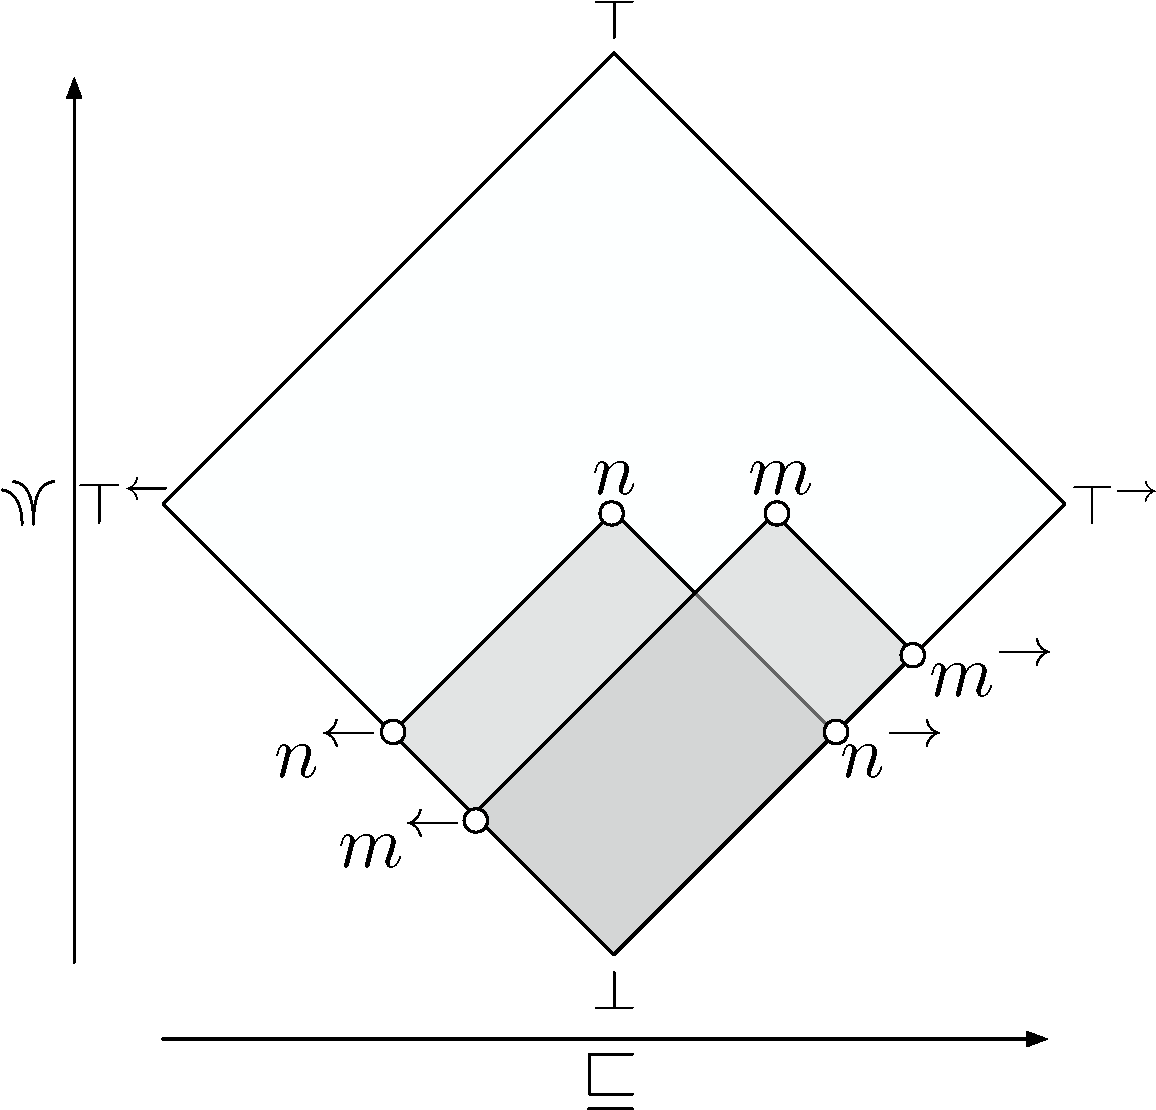
\includegraphics[scale=0.25]{Illustrations/multi-node.pdf}
    \caption{As nodes $n$ and $m$ performs computations their current labels will float from the left-most point to the right-most point in the lattice.}
    \label{fig:node-info-flow}
\end{figure}

\subsection{Remote Procedure Calls}
Nodes in \lang{} communicate by remote invocation of functions on different machines. We annotate functions with the node on which the function should be evaluated. That is, the application $\app{(\abs{n}{p}{x}{\expr})}{\expr'}$ denotes a function $\abs{n}{p}{x}{\expr}$ located on machine $n$ should be evaluated with argument $\expr'$ and the returned expression will be given label $p$. For instance, the expression
\begin{lstlisting}
((*@$\lambda^{n}_{p}$@*) x . not x) b >>= (*@$\lambda^{m}_{m}$@*) y . unlabel y
\end{lstlisting}
computes the negation of the boolean $b$ on node $n$ and returns the result as a labeled value with label $p$, which is then unlabeled on node $m$. After receiving the labeled value computed by node $n$, node $m$ needs to unlabel the value to use it. The unlabel command checks that $p \flowsto \conf{n}$.

\subsection{Proof search}
In order to prove queries of the form $p \flowsto \conf{n}$ a distributed proof search is performed. The two most important rules for the proof search judgment is the rule for using delegations, and the rule for forwarding trust checking to other nodes in the system. We discuss these two rules informally here.

\paragraph{Delegations}
Delegations of the form $\lb{r}{p \actsfor q}$ (pronounced $r$ \emph{says that} $p$ \emph{acts for} $q$) can be used by a proof search on a node $n$ when $r \flowsto \conf{n}$\footnote{The actual judgment requires other trust relationships to hold, but we omit these for now. The rule will be given formally in Section~\ref{sec:calculus}.}. We say that the delegation $\lb{r}{p \actsfor q}$ is \emph{labeled} with label $r$. Using a delegation in a proof search will raise the current label by the label of the delegation, and thus fine-grained control of how delegations are used is important. For this reason \lang{} uses \emph{strategies}, which are lists of principals, to specify which delegations can be used in a proof, and in which order. For instance, if the delegation $\lb{r}{p \actsfor q}$ is ``known'' by node $n$ and $n$ is evaluating the expression
\begin{lstlisting}
withStrategy [s, r, t] (p (*@$\actsfor$@*) q)
\end{lstlisting}
the node will first search for the delegations with a label that flows to $s$. Assuming this fails, delegations with a label that flows to $r$ will be used, and if $r \flowsto \conf{n}$ the delegation can be used to complete the proof search. This illustrates how \lang{} performs fine-grained proof search with custom strategies for handling delegations.

\paragraph{Forwarding}
A node $n$ can forward the checking of trust checking to a node $m$ when $n$'s current label flows to $\conf{m}$. Combining uses of this rule with delegations, this allows a node to use delegations local to other nodes in the system. For instance, a server $s$ can represent users authorized by $s$ by delegating ownership projections $\owner{s}{u}$ for every authorized user $u$. The delegation $\lb{\integ{s}}{\owner{s}{u} \actsfor \mathsf{users}}$ then represents that user $u$ is authorized\footnote{This encoding of group membership prevents \emph{delegation loophole} as defined in \cite{Arden:2015:FA:2859845.2859998}. We omit the details of ownership projections as they are not important for this motivating example.}. Another user $u'$ can then evaluate
\begin{lstlisting}
withStrategy [(*@$\integ{s}$@*)] ((*@$\owner{s}{u} \actsfor \mathsf{users}$@*))
\end{lstlisting}
and forward the proof search to the server, which will succeed and return a positive answer back to $u'$.

\section{A calculus for \lang}\label{sec:calculus}

This section introduces a formalization of the \lang{} language. We first introduce the syntax and semantics of the language and afterward present the judgment for deriving trust between principals in the language. Finally, this section presents a type system for \lang. 

\subsection{Syntax}

Figure~\ref{fig:language-syntax} shows the syntax of \lang. The meta-variable $\val$ ranges over terms, which include boolean literals, the unit value, runtime representations of principals, addresses and variables, abstractions $\abs{n}{\lb{p}{\type}}{x}{\expr}$, which are parameterized over the principal name $n$ on which to evaluate the expression $\expr$, and the principal $p$ representing the label on the value returned from invoking the abstraction. To simplify the presentation of the semantics abstractions are annotated with the type of $\expr$. Finally, the language includes lists using $\nil$ and $\consop$ (pronounced ``cons'') to model strategies.

Expressions are ranged over by the meta-variable $\expr$ and include terms, applications, projections, elimination of booleans and lists, recursive functions, monadic expressions using $\returnkw$ and $\bindop$, allocation, reading and writing of references. Following LIO \cite{SRMMlio}, the language supports operations for labeling and unlabeling expressions, and the operation $\tolabeledkw$ for controlling label-creep \cite{SRMMlio}. The operations $\getlabel$ and $\getclearance$ returns the current label and clearance of the computational context respectively, and $\labelofkw$ returns the label of a labeled value. Following \cite{Moore:2016:EAC:2983990.2984021} the scope of delegations is ``fluid'' and the operation $\withscopekw$ creates a new fluid scope. Strategies (introduced later in this section) are introduced using the $\withstrategykw$ operation, and the current strategy can be obtained using $\getstrategy$. Finally, delegations can be added and queried. The shaded regions describe syntax not part of the surface language, but rather constructs used during evaluation.

Finally, types are ranged over by the meta-variable $\type$ and include standard types like the boolean type; the unit type; as well as function-, list- and product types. Non-standard types include the type of FLAM principals, the type of labeled values, the type of LIO computations as well as location-aware reference types.

\begin{figure*}
    \centering
    \begin{tabular}{l}
         $\val ::= \true \mid \false \mid () \mid p \mid \addr \mid x \mid \abs{n}{\lb{p}{\type}}{x}{\expr} \mid (\expr, \expr) \mid \cons{\expr}{\expr} \mid \nil \mid \graybox{\lb{p}{\expr}} \mid \graybox{\lio{\expr}}$ \\
         $\begin{aligned}[t]
         \expr &::= \val \mid \app{\expr}{\expr} \mid \proj{i}{\expr} \mid \ifexpr{\expr}{\expr}{\expr} \mid \case{\expr}{\expr}{\expr} \mid \fix{\expr} \mid \return{\expr} \mid \bind{\expr}{\expr} \\ &\quad \mid
         \new{\expr}{\expr} \mid \readref{\expr} \mid \writeref{\expr}{\expr} \mid \Label{\expr}{\expr} \mid \unlabel{\expr} \mid
         \tolabeled{\expr}{\expr} \mid \getlabel \\ &\quad \mid \getclearance \mid \labelof{\expr} \mid \withscope{\expr} \mid \expr \actsfor \expr \mid \withstrategy{\expr}{\expr} \\ &\quad \mid \adddelegate{\expr}{\expr}{\expr} \mid \getstrategy \mid \graybox{\wait{n}[\type]} \mid \graybox{\resetstrategy{\overline{p}}{\expr}} \\ &\quad \mid \graybox{\resetTolabeled{p}{q}{\expr}} \mid \graybox{\resetscope{\scope}{\expr}}
         \end{aligned}$ \\
         $\type ::= \bool \mid \unit \mid \func{\type}{\type} \mid \listtype{\type} \mid \pair{\type}{\type} \mid \labeltype \mid \labeled{\type} \mid \liotype{\type} \mid \reftype[n]{\type}$ \\
    \end{tabular}
    \caption{The \lang{} language}
    \label{fig:language-syntax}
\end{figure*}

\subsection{Semantics}\label{sec:semantics}
The semantics of \lang{} can be split into two judgments: Local reduction rules, which evaluate an expression on a specific node; and global reduction rules, which models remote procedure calls (RPC) and returns. We first present the local reduction rules.

\paragraph{Local semantics}
The semantics of local reduction rules is given by a structured operational semantics with evaluation contexts \cite{Felleisen:1988:TPF:73560.73576}. We elide the definition of the evaluation context, as this is mostly standard.

We further split the local reduction rules into two categories: Pure reduction rules $\steppure{\expr}{\expr'}$ which reduces expressions independent of memories and independent of which principal is evaluating the expression. The pure reduction rules are seen in Figure~\ref{fig:pure-reductions}. Pure reductions include packing terms into monadic contexts, monadically binding terms, recursive applications, projecting pairs, eliminating booleans and lists and obtaining the label of a labeled value.

\begin{figure}
    \centering
    \begin{mathpar}
    \inferrule{}{\steppure{\efill{\return{\val}}} {\efill{\lio{\val}}}}
    \and
    \inferrule{}{\steppure{\efill{\bind{\lio{\val}}{\expr}}}{\efill{\app{\expr}{\val}}}}
    \and
    \inferrule{}{\steppure{\efill{\fix{\expr}}}{\efill{\app{\expr}{(\fix{\expr})}}}}
    \and
    \inferrule{}{\steppure{\efill{\proj{i}{(\val_1, \val_2)}}}{\efill{\val_i}}}
    \and
    \inferrule{}{\steppure{\efill{\ifexpr{b}{\expr_{\true}}{\expr_{\false}}}}{\efill{\expr_b}}}
    \and
    \inferrule{}{\steppure{\efill{\case{\nil}{\expr_1}{\expr_2}}}{\efill{\expr_1}}}
    \and
    \inferrule{}{\steppure{\efill{\case{(\cons{\expr_\hd}{\expr_\tl})}{\expr_1}{\expr_2}}}{ \efill{\app{\app{\expr_2}{\expr_\hd}}{\expr_\tl}}}}
    \and
    \inferrule{}{\steppure{\efill{\labelof{(\lb{p}{\expr})}}}{\efill{p}}}
    \and
    \inferrule{\steppure{\expr}{ \expr'}}{\steppure{\efill{\expr}}{\efill{\expr'}}}
    \end{mathpar}
    \caption{Pure reductions for \lang.}
    \label{fig:pure-reductions}
\end{figure}

The remaining local reductions all depend either on memory or on the identity of the principal which evaluates the expression. We denote these as \emph{monadic reductions}.

Before introducing the monadic small-step local reduction, we introduce the remaining necessary concepts: First, a store $\store: \Addr \partialto \val$ is a partial mapping from addresses to terms, and we write the empty store as $\varnothing$. A local configuration is a pair $\config{\store}{\overline{\expr}}$ consisting of a store $\store$ and a stack of expressions $\overline{\expr}$. We use stacks of expressions to handle incoming remote procedure calls (RPC) that ``interrupts'' the current computation to evaluate the RPC. A global environment $\env: \Nameset \to \sigma$ is a mapping from names to local environments $\sigma$. A local environment $(\lblkw, \scope, \strategy)$ contains the current label ($\lblkw$), the set of delegations local to the principal ($\scope$) and the current strategy of the principal. ($\strategy$). We use record notation for these and write $\sigma.\lblkw$, $\sigma.\scope$ and $\sigma.\strategy$ respectively. We let $\emptyenv$ denote the initial global environment satisfying $\emptyenv(n) = (\conf{\bot} \conj \integ{n}, \nil, \nil)$. That is, the initial global environment maps all names to an initial local environment with a current label $\conf{\bot} \conj \integ{n}$, the empty list of delegations and the empty strategy. While this notation conflicts with the empty store, the context always allows for disambiguation.

The small-step relation is written $\step{n; \env}{\config{\store}{\expr}}{\config{\store'}{\expr'}}{\sigma}$ and should be read as ``the global environment is $\env$ and machine $n$ performs a single reduction and updates its local environment from $\env_n$ to $\sigma$''.

Figure~\ref{fig:monadic-reductions} in the appendix shows the local reduction rules. Most of the rules verify some trust relationship between principals, written $\actsforquery{n; \env}{p}{q}{\level}$ and can be read as ``node $n$ proves that $p$ acts for $q$ and uses information labeled up to $\level$ in the process''. We defer the discussing this judgment until Section~\ref{subsec:deriving-trust}.

Rule \ruleref{E-Lift-Pure} lifts pure reductions to monadic reductions. Due to the structure of our evaluation contexts ($\ectx \hole ::= \ldots \mid \ectx \hole ; \overline{\expr}$) an expression can reduce at the top of the expression stack only. This is why pure reductions are defined only for single expressions, while the monadic reductions work over lists of expressions. Rules \ruleref{E-Get-Label} and \ruleref{E-Get-Clearance} returns the current label or clearance of the principal upon which the expression is being evaluated. Rule \ruleref{E-App} applies a function to an argument and labels the resulting value with the given principal. This choice may seem strange: Why deviate from the traditional semantics of function application? The answer is that with this approach we can combine local function calls and RPC into the same typing rule, and thus simplify the proofs. However, it is straightforward to extend the language with different syntactic constructions for local function application. It would also be straightforward to apply syntactic sugar that unlabels the returned value in case of local function applications.

Rules \ruleref{E-New}, \ruleref{E-Read}, \ruleref{E-Write}, \ruleref{E-Label} and \ruleref{E-Unlabel} are all equivalent to the ones presented in \cite{SRMMlio}, but now also take into account the possible information-flows arising via deriving trust relationships \cite{Arden:2015:FA:2859845.2859998}. Rules \ruleref{E-ToLabeled-1} and \ruleref{E-ToLabeled-2} evaluates an expression $\expr$, but once $\expr$ is evaluated to a term $\val$, the current label is restored to its state before evaluation of $\expr$ began. This operation helps prevent label creep \cite{SRMMlio}, and security guarantees can be reestablished by labeling $\val$. Note that the presentation of this operation is different from \cite{SRMMlio} in that we avoid interleaving small-step and big-step operations, which simplifies the proofs considerably.

Rules \ruleref{E-Acts-For-True} and \ruleref{E-Acts-For-False} queries the trust relationship between two given principals. Rules \ruleref{E-With-Scope} and \ruleref{E-Reset-Scope} introduce and eliminate a fluid scope respectively. Rules \ruleref{E-With-Strategy} introduces a new strategy and evaluates an expression in the lexical scope of the new strategy. Rule \ruleref{E-Reset-Strategy} eliminates the strategy once the expression reduces to a term. Finally, \ruleref{E-Assume} adds a new delegation. This rule uses the voice operator $\voicekw$ defined in Section~\ref{sec:background} to ensure that the computational context has sufficient integrity to delegate trust on behalf of $q$.

Figure~\ref{fig:use-case-for-fluid-scope} demonstrates the usefulness of fluid scoping for delegations. $\mathsf{Alice}$ invokes a function on $\mathsf{Bob}$'s machine that grants another function (given as an argument) the authority to read Bob's confidential information. In addition, Bobs enforces the policy that the function is only called once. Due to the $\withscopekw$ construct, the additional authority is only given to the function passed as an argument. Any other function will still not be able to read Bob's confidential information.

\begin{figure}
\centering
\begin{lstlisting}
((*@$\lambda^{\mathsf{Alice}}$@*) _ . [...]
  let g = ((*@$\lambda^{\mathsf{Bob}}$@*) f .
              bref := new (*@$\integ{\mathsf{Bob}}$@*) true
              withScope (
                assume (*@$\conf{\mathsf{Alice}}$@*) (*@$\actsfor$@*) (*@$\conf{\mathsf{Bob}}$@*) @ (*@$\integ{\mathsf{Bob}}$@*)
                return ((*@$\lambda^{\mathsf{Alice}}$@*) x . 
                           b <- !bref
                           bref := false
                           if b then f x else false))) aliceCode
  in g bobSecret) ()
\end{lstlisting}
\caption{Bob grants a function supplied by Alice with authority to read Bob's confidential information once. }
\label{fig:use-case-for-fluid-scope}
\end{figure}

To see how strategies can be used to prevent label creep consider the following scenario: At some point the query $p \actsfor q$, where $p, q \in \Nameset$ is issued. The current set of delegations is $\scope = \{ \lb{p_1}{x_1}, \dots, \lb{p_n}{x_n} \}$. As each $\lb{p_i}{x_i}$ is labeled pair it is not possible to inspect these without unlabeling the pair and raise the current label. We now want to unlabel as few of these as possible to prove that $p \actsfor q$. Strategies give the programmer first-class control over which delegations are unlabeled, and in which order. For instance, if the programmer knows that there will always be a delegation $\lb{r}{p \actsfor q}$ or $\lb{s}{p \actsfor q}$, the strategy $\left[ r, s \right]$ can be set, which firsts checks if a proof can be found using only delegations with a label that flows to $r$. If that fails, delegations with a label that flows to $s$ are checked. In this way, the programmer can choose the strategy that minimizes the label creep for each trust query.

\paragraph{Global semantics}
A global configuration is a triple $\gconfig{n}{\env}{S}$ consisting of a node $n \in \Nameset$ denoting which machine is currently reducing an expression, a global environment $\env$, and a mapping $S$ from names to local configurations. Figure~\ref{fig:global-steps} presents the reduction rules for global configurations. Rule \ruleref{G-Step-Local} lifts a local reduction to a global reduction, and rules \ruleref{G-Step-App} and \ruleref{G-Step-Ret} handle remote procedure calls and returns respectively. When node $n$ sends an RPC to node $m$, we call $n$ the source machine and $m$ the target machine. The global reduction rule is written as $\gconfig{n}{\env}{S} \gstepsto \gconfig{n'}{\env'}{S'}$ and can be read as ``Machine $n$ updates the environment $\env$ to $\env'$, updates the local environments $S$ to $S'$, and transfers control to machine $n'$''. We write the reflexive, transitive closure of $\gstepsto$ as $\gstepstos$.

We now explain how to model RPC. First, \ruleref{G-Step-App} transfers control to the target machine, and the computation is wrapped in a $\tolabeledkw$ construct at the top of the execution stack on the target machine to prevent the evaluation of the expression from raising the current label. Finally, the evaluation on source machine is suspended. Second, Rule \ruleref{G-Step-Ret} returns control to a suspended source machine when the top of the execution stack on the target machine has reduced to a term.

The final rule, \ruleref{G-Step-Stop} halts the execution when the last machine has reduced its expression to a term. We use the notation $\bullet(S)$ to mean $S = \config{\store}{\bullet}$ for some store $\store$.

Note that the computation is decentralized, and multiple machines with different resources stored in their memories can cooperate and invoke each other, but the semantics is still deterministic in that only one expression is reducible at any point. This determinism excludes internal timing leaks and other attacks usually found in concurrent systems \cite{Smith:1998:SIF:268946.268975, Muller:2012:TPS:2384616.2384621}, while still allowing multiple nodes to share computation.

\begin{figure*}
\centering
\begin{mathpar}
\inferrule[G-Step-Local]{\step{n; \env}{S_n}{S'}{\sigma}}{\gconfig{n}{\env}{S} \gstepsto \gconfig{n}{\extend{\env}{n}{\sigma}}{\extend{S}{n}{S'}}}
\and
\inferrule[G-Step-App]{\level_n = \env_n.\lblkw \and \level_m = \env_m.\lblkw \and S_m = \config{\store_m}{\overline{\expr_m}} \and \nopostflowstoquery{m; \env}{\level_n \join \level_m}{m} \\\\ S_n = \config{\store_n}{\efill{\app{(\abs{m}{\lb{p}{\type}}{x}{\expr_n})}{\expr_n'}}} \and S_n' = \config{\store_n}{\efill{\wait{m}[\type]}} \\\\ S_m' = \config{\store_m}{(\resetTolabeled{\level_m}{p}{(\expr_n[\expr_n' / x])}) ; \overline{\expr_m}}}{\gconfig{n}{\env}{S} \gstepsto \gconfig{m}{\extend{\env}{m}{\extend{\env_m}{\lblkw}{\level_n \join \level_m}} }{\extends{S}{n \mapsto S_n', m \mapsto S_m'}}}
\and
\inferrule[G-Step-Ret]{S_n = \config{\store_n}{\efill{\wait{m}[\type]}} \and S_m = \config{\store_m}{\val ; \overline{\expr_m}} }{\gconfig{m}{\env}{S} \gstepsto \gconfig{n}{\env}{\extends{S}{n \mapsto \config{\store_n}{\efill{\val}}, m \mapsto \config{\store_m}{\overline{\expr_m}}}}}
\and
\inferrule[G-Step-Stop]{\forall n \in \Nameset \setminus \{m\}~.~ \termsym(S_n) \and S_m = \config{\store_m}{\val ; \termsym}}{\gconfig{m}{\env}{S} \gstepsto[][] \gconfig{m}{\env}{\extend{S}{m}{\config{\store_m}{\termsym}}}}
\end{mathpar}
\caption{Semantics of global steps}
\label{fig:global-steps}
\end{figure*}

\subsection{Deriving trust relationship in \lang}\label{subsec:deriving-trust}
\begin{figure}
    \centering
    \begin{mathpar}
    \inferrule[Bot]{}{\actsforquery{C}{p}{\bot}{\botinfoflow}}
    \and
    \inferrule[Top]{}{\actsforquery{C}{\top}{p}{\botinfoflow}}
    \and
    \inferrule[Refl]{}{\actsforquery{C}{p}{p}{\botinfoflow}}
    \and
    \inferrule[Hyp]{(p \actsfor q) \in \Assumps}{\actsforquery{C}{p}{q}{\botinfoflow}}
    \and
    \inferrule[Proj]{\actsforquery{C}{p}{q}{\level}}{\actsforquery{C}{\authproj{p}}{\authproj{q}}{\level}}
    \and
    \inferrule[ProjR]{}{\actsforquery{C}{p}{\authproj{p}}{\botinfoflow}}
    \and
    \inferrule[Own-1]{\actsforquery{C}{o}{o'}{\level_1} \\\\ \actsforquery{C}{p}{p'}{\level_2}}{\actsforquery{C}{\owner{o}{p}}{\owner{o'}{p'}}{\level_1 \join \level_2}}
    \and
    \inferrule[Own-2]{\actsforquery{C}{o}{o'}{\level_1} \\\\ \actsforquery{C}{p}{\owner{o'}{p'}}{\level_2}}{\actsforquery{C}{\owner{o}{p}}{\owner{o'}{p'}}{\level_1 \join \level_2}}
    \and
    \inferrule[Conj-L]{j \in \{ 1, 2 \} \\\\ \actsforquery{C}{p_j}{p}{\level}}{\actsforquery{C}{p_1 \conj p_2}{p}{\level}}
    \and
    \inferrule[Conj-R]{\actsforquery{C}{p}{p_1}{\level_1} \\\\\ \actsforquery{C}{p}{p_2}{\level_2}}{\actsforquery{C}{p}{p_1 \conj p_2}{\level_1 \join \level_2}}
    \and
    \inferrule[Disj-L]{\actsforquery{C}{p_1}{p}{\level_1} \\\\\ \actsforquery{C}{p_2}{p}{\level_2}}{\actsforquery{C}{p_1 \disj p_2}{p}{\level_1 \join \level_2}}
    \and
    \inferrule[Disj-R]{j \in \{ 1, 2 \} \\\\ \actsforquery{C}{p}{p_j}{\level}}{\actsforquery{C}{p}{p_1 \disj p_2}{\level}}
    \and
    \inferrule[Trans]{\actsforquery{C}{p}{q}{\level_1} \\\\ \actsforquery{C}{q}{r}{\level_2}}{\actsforquery{C}{p}{r}{\level_1 \join \level_2}}
    \and
    \inferrule[Del]{\mathsf{ss} = \env_n . \strategy \\\\ \actsforquerysmany{C}{\mathsf{ss}}{p}{q}{\level}}{\actsforquery{C}{p}{q}{\level}}
    \and
    \inferrule[Fwd]{\flowstoquery{C}{\env_n . \lblkw}{\conf{m}}{\level_1} \\\\ \actsforquery{\Assumps; m; \extend{\env}{m}{\extend{\env_m}{\strategy}{\env_n.\strategy}}}{p}{q}{\level_2} }{\actsforquery{C}{p}{q}{\level_1 \join \level_2}}
    \end{mathpar}
    \caption{Acts for judgment of \lang. The meta-variable $C$ abbreviates $\Assumps; n; \env$}
    \label{fig:act-for-judgment}
\end{figure}

\lang{} allows, in the style of FLAM \cite{Arden:2015:FA:2859845.2859998}, the trust relationship between principals to be changed and queried dynamically throughout the evaluation of a program. We show how the ideas from FLAM on how to provide guarantees of confidentiality and integrity can be incorporated into the floating-label model of LIO. Figure~\ref{fig:act-for-judgment} shows how the judgment $\actsforquery{\Assumps; n; \env}{p}{q}{\level}$ derives trust relationships between principals. Intuitively $\actsforquery{\Assumps; n; \env}{p}{q}{\level}$ means that node $n$ has to raise its current floating label to be at least $\level$ in order to use the information that $q$ trusts $p$, assuming hypotheses $\Assumps \subseteq \mathcal{P} \times \mathcal{P}$ and global environment $\env$. We write $\actsforquery{n; \env}{p}{q}{\level}$ to mean $\actsforquery{\varnothing; n; \env}{p}{q}{\level}$.

Many rules translate directly from FLAM, except for (1) using delegations and (2) querying remote nodes for trust relationships. This discrepancy is because upper bound on the label of usable delegations in FLAM is given as ``input'' to the judgment, while in \lang{} the upper bound is part of the ``output'' of the judgment.\footnote{That the upper bound on the delegation labels is an ``input'' to the judgment can be seen in the $F\lambda$ calculus \cite{flamtr} where delegation labels appear in the surface syntax of expressions.}

Rule \ruleref{Bot} says that the element $\bot$ trusts any principal, and that deriving this trust requires information up to level $\botinfoflow$. Dually, \ruleref{Top} states that any principal trusts $\top$, and \ruleref{Refl} states that any element trusts itself. Rule \ruleref{Hyp} states that any hypothesis can be used to derive trust without raising the current label any further. This use of assumptions is an instance of a checked endorsement \cite{Chong:2007:SWA:1294261.1294265, DBLP:journals/corr/abs-1107-5594}, and is discussed later in this section. Rule \ruleref{Proj} expresses that applying projections preserve trust between principals and \ruleref{ProjR} states that a principal is at least as trusted as the projected principal. Rules \ruleref{Own-1} and \ruleref{Own-2} derives trust between ownership projections. First, \ruleref{Own-1} shows that trust between principals imply trust between owned principals, and \ruleref{Own-2} states that, if an ownership projection $\owner{o'}{p'}$ trusts a principal $p$ then another ownership principal $\owner{o}{p}$ also trusts $\owner{o'}{p'}$, but only if the the owner $o'$ trusts $o$. Rules \ruleref{Conj-L}, \ruleref{Conj-R}, \ruleref{Disj-L}, and \ruleref{Disj-R} correspond to the usual lattice rules for joins and meets, and \ruleref{Trans} ensures that the trust relation is transitive. Rule \ruleref{Fwd} expresses how a node $n$ can query another node $m$ for a trust relationship, but only if $n$ allows the information that caused $n$ to contact $m$ to be learned by $m$. Furthermore, the searching strategy used by $n$ should also be used by $m$ as otherwise, it would make local reasoning about trust relationship queries impossible without knowing the strategies of every node in the system.

Finally, rule \ruleref{Del} expresses how delegations can be used to derive trust. The judgment uses the search strategy $\mathit{ss}$ to control how the information-flow lattice is searched: If $\mathit{ss} = \lbrack s_1, \dots, s_n \rbrack$ delegations with labels that flow to $s_1$ are unlabeled. If that fails, delegations that flow to $s_2$ are unlabeled. This process continues until either the query is proven, or every principal in the strategy is used.

\begin{figure}
    \centering
    \begin{mathpar}
    \inferrule[Del-1]{\lb{\level}{p \actsfor q} \in \env.\scope \\\\ \flowstoquery{\Assumps, p \actsfor q; n; \env}{\level}{s}{\level'} \and \flowstoquery{\Assumps, p \actsfor q; n; \env}{\level'}{s}{\botinfoflow}}{\actsforquerysmany{\Assumps; n; \env}{\mathsf{s}::\mathsf{ss}}{p}{q}{s}}
    \and
    \inferrule[Del-2]{\lb{\level}{p \actsfor q} \in \env.\scope \implies \\\\ (\forall \level'~.~\notflowstoquery{\Assumps, p \actsfor q; n; \env}{\level}{s}{\level'} \, \vee \\\\ \flowstoquery{\Assumps, p \actsfor q; n; \env}{\level}{s}{\level'} \, \wedge \notflowstoquery{\Assumps, p \actsfor q; n; \env}{\level'}{s}{\botinfoflow}) \\\\
    \actsforquerysmany{\Assumps; n; \env}{\mathsf{ss}}{p}{q}{\level'}
    }{\actsforquerysmany{\Assumps; n; \env}{\cons{\mathsf{s}}{\mathsf{ss}}}{p}{q}{\level' \join s}}
    \end{mathpar}
    \caption{Auxiliary judgment for using delegations when proving an acts for query in \lang.}
    \label{fig:act-for-judgment-del}
\end{figure}

 Figure~\ref{fig:act-for-judgment-del} formalizes this idea, where the first element $s$ in the strategy $\mathit{ss}$ that successfully derives the trust relationship terminates the proof search. Rule \ruleref{Del-1} terminates the proof search if a delegation that proves the query is found, as long as the delegation label can be proven to flow to the strategy principal. Note that this might require further use of delegations, and thus an additional check needs to be performed to verify that the information used is less than the strategy. This checking could potentially continue ad infinitum, so we apply a pragmatic approach and require this check not to use any delegations labeled higher than $\botinfoflow$. Section~\ref{sec:case-studies} motivates this decision, which shows several interesting examples that can all be implemented using this simplified checking mechanism.

Rule~\ruleref{Del-2} checks that the label of all delegations involving the same principals as the goal either (1) cannot be proven to flow to the strategy or (2) can be proven to flow to the strategy, but not without using delegations whose label does not flow to the strategy.

Note that, when checking if a delegation can be used in rules~\ruleref{Del-1} and \ruleref{Del-2} the hypotheses set $\Assumps$ is extended to include the trust relationship that is in the process of being proven to hold. This usage of hypotheses is a form of checked endorsement which was also noted to be a useful extension to the Jif programming language \cite{Chong:2007:SWA:1294261.1294265}.
To see the effect of this style of reasoning, assume $\Nameset = \{n\}$ and consider the query $\flowstoquery{n; \env}{p}{q}{\level}$ where $\env_n = (\botinfoflow, \scope, \lbrack q \rbrack)$ and $\scope = \{\lb{p}{(\conf{q} \conj \integ{p} \actsfor \conf{p} \conj \integ{q})} \}$. This query is equivalent to $\actsforquery{n; \env}{\conf{q} \conj \integ{p}}{\conf{p} \conj \integ{q}}{\level}$, so applying \ruleref{Del} and \ruleref{Del-1} the goal reduces to proving $\flowstoquery{p \flowsto q; n; \env}{p}{q}{\level'}$ for some $\level'$, which is the exact same query we started out with! However, now we have the hypothesis $p \flowsto q$, and the goal follows by applying \ruleref{Hyp}.

If the condition $\flowstoquery{\{p \flowsto q\}; n; \emptyenv}{p}{q}{\botinfoflow}$ was changed to the ``naive'' condition $\flowstoquery{n; \env}{p}{q}{\level'}$, that is, no assumptions was added when checking that the label on the delegation $\lb{p}{p \flowsto q}$ flows to the strategy principal $q$, this trust relationship could not be proven in any finite derivation. While this situation might appear synthetic, it was noted in several of the case studies described in Section~\ref{sec:case-studies}.

We end this section with an example of a query that morally should hold, but which cannot be justified using our trust judgment. Given the following set of delegations $\scope = \{ \lb{c}{a \actsfor b}, \lb{\botinfoflow}{c \flowsto d} \}$, the judgment $\actsforquery{n; \env}{a}{b}{d}$ holds for $\env = (\lblkw, \scope, \lbrack d \rbrack)$ using rule \ruleref{Del} and \ruleref{Del-1} with the fact that $\flowstoquery{a \actsfor b; n; \env}{c}{d}{\botinfoflow}$ and $\flowstoquery{a \actsfor b; n; \env}{\botinfoflow}{\botinfoflow}{\botinfoflow}$. Similarly, the same judgment holds if $\scope = \{ \lb{c}{a \actsfor b}, \lb{e}{c \flowsto d}, \lb{\botinfoflow}{e \flowsto d} \}$ using the same rules and the facts that $\flowstoquery{a \actsfor b; n; \env}{c}{d}{e}$ and $\flowstoquery{a \actsfor b; n; \env}{e}{d}{\botinfoflow}$. But if $\scope = \{ \lb{c}{a \actsfor b}, \lb{e}{c \flowsto d}, \lb{f}{e \flowsto d}, \lb{\botinfoflow}{f \flowsto d} \}$ the same query cannot be proven since, although $\lb{c}{a \actsfor b} \in \env.\scope$ and $\flowstoquery{a \actsfor b; n; \env}{c}{d}{e}$ it is not the case that $\flowstoquery{a \actsfor b; n; \env}{e}{d}{\botinfoflow}$.

\subsection{A type system for \lang.}
Since \lang{} controls information-flows via dynamic checks, the type system for \lang{} is straightforward. We write $\hastype{n; \tenv}{\expr}{\type}$ when expression $\expr$ can be given type $\type$ in a global type environment $\tenv: \Nameset \to (\Var \to \type)$ on machine $n$. Figure~\ref{fig:type-judgment} shows excerpts of this judgment. Rule \ruleref{T-Principal} states that principals have type $\labeltype$, and \ruleref{T-Var} states that variable types are given by the global type environment $\tenv$. Rule \ruleref{T-Ref} simplifies the statement of Theorem~\ref{thm:preservation} by having the typing environment denote the type of both variables and addresses. We say an address $\addr$ belongs to node $n$ if $\hastype{m; \tenv}{\addr}{\reftype[n]{\type}}$ for some $m$. Rule \ruleref{T-Abs} states that an abstraction has a function type and that, the typing environment for node $m$ is used when checking the type of the body, where $m$ is the target machine. Rule \ruleref{T-Lab} states that labeled expressions have labeled types. Rules \ruleref{T-Lio}, \ruleref{T-Return} and \ruleref{T-Bind} are standard typing rules for monadic expressions. Rules \ruleref{T-New} states that, when a reference is allocated on a node $n$ the type of the address returned will belong to $n$. Rule \ruleref{T-Read} states that a reference can only be read on a machine on which the address belongs. Finally, \ruleref{T-Wait} states that the type attached to a waiting expression is the type of the expression. The rules \ruleref{T-Wait} and \ruleref{T-Abs} are closely connected in that an RPC will evaluate an abstraction to a waiting expression, meaning that the typing rules for these expressions should match.

\paragraph{Store typing}
Given a global typing environment $\tenv$ we write $\wf{m; \tenv}{\store}$ if, for all $\addr$ such that $\store(\addr) = \lb{p}{\expr}$ and $\tenv_m(\addr) = \reftype[n]{\type}$ it holds that $\hastype{n; \tenv}{\expr}{\type}$. We write $\hastype{n; \tenv}{\config{\store}{\overline{\expr}}}{\overline{\type}}$ if $\wf{n; \tenv}{\store}$ and $\hastype{n; \tenv}{\expr_i}{\type_i}$ for $i = 1, \dots, n$ and $\overline{\expr} = \expr_1 \cdots \expr_n$ and $\overline{\type} = \type_1 \dots \type_n$. We lift this definition to global configurations and write $\hastype[m]{\tenv}{\gconfig{n}{\env}{S}}{\overline{\type}}$ if for all $n' \in \Nameset$ there exists a type $\overline{\type}'$ such that $\hastype{n'; \tenv}{S_{n'}}{\overline{\type}'}$, and furthermore, when $n' = m$ we have $\overline{\type}' = \overline{\type}$.

\paragraph{Preservation}
As the program allocates references during evaluation, the typing environment needs to incorporate these addresses accordingly. Thus Theorem~\ref{thm:preservation} shows that, if a configuration is well-typed and takes a single step, there exists a global typing environment, which is an extension of the old typing environment, such that the new configuration is well-typed.

\begin{theorem}[Preservation]\label{thm:preservation}
If $\hastype[m]{\tenv}{\gconfig{n}{\env}{S}}{\overline{\type}}$ and $\gconfig{n}{\env}{S} \gstepsto \gconfig{n'}{\env'}{S'}$ then there exists $\tenv' \supseteq \tenv$ and $\overline{\type}$ such that either $\overline{\type}' \leq \overline{\type}$ or $\overline{\type} \leq \overline{\type}'$ and $\hastype[m]{\tenv'}{\gconfig{n'}{\env'}{S'}}{\overline{\type}'}$.
\end{theorem}

We write $\overline{\type_1} \leq \overline{\type_2}$ to mean that $\overline{\type_1}$ is a \emph{prefix} of $\overline{\type_2}$. So Theorem~\ref{thm:preservation} states that the global reduction semantics steps to a global configuration which type is either a prefix or a suffix of the original type. The statement in the technical report~\cite{techreport} is stronger: It proves that $\overline{\type}' \leq \overline{\type}$ when $\gconfig{n}{\env}{S} \gstepsto \gconfig{n'}{\env'}{S'}$ is an application of \ruleref{G-Step-Ret} and $\overline{\type} \leq \overline{\type}'$ when $\gconfig{n}{\env}{S} \gstepsto \gconfig{n'}{\env'}{S'}$ is an application of \ruleref{G-Step-App}, and $\overline{\type} = \overline{\type}'$ otherwise.

\begin{figure}
\centering
\begin{mathpar}
\inferrule[T-Principal]{~}{\hastype{n; \tenv}{p}{\labeltype}}
\and
\inferrule[T-Var]{\tenv_n(x) = \type}{\hastype{n; \tenv}{x}{\type}}
\and
\inferrule[T-Ref]{\tenv_n(\addr) = \reftype[n]{\type}}{\hastype{n; \tenv}{\addr}{\reftype[n]{\type}}}
\and
\inferrule[T-Abs]{\hastype{m; \tenv, x : \type_1}{\expr}{\liotype{\type_2}} \\\\ \type = \func{\type_1}{\liotype{(\labeled{\type_2})}}}{\hastype{n; \tenv}{\abs{p}{\lb{m}{\type_2}}{x}{\expr}}{\type}}
\and
\inferrule[T-Lab]{\hastype{n; \tenv}{\expr_2}{\type} \\\\ \hastype{n; \tenv}{\expr_1}{\labeltype}}{\hastype{n; \tenv}{\lb{\expr_1}{\expr_2}}{\labeled{\type}}}
\and
\inferrule[T-Lio]{\hastype{n; \tenv}{\expr}{\type}}{\hastype{n; \tenv}{\lio{\expr}}{\liotype{\type}}}
\and
\inferrule[T-Return]{\hastype{n; \tenv}{\expr}{\type}}{\hastype{n; \tenv}{\return{\expr}}{\liotype{\type}}}
\and
\inferrule[T-Bind]{\hastype{n; \tenv}{\expr_1}{\liotype{\type_1}} \\\\ \hastype{n; \tenv}{\expr_2}{\func{\type_1}{\liotype{\type_2}}}}{\hastype{n; \tenv}{\bind{\expr_1}{\expr_2}}{\liotype{\type_2}}}
\and
\inferrule[T-New]{\hastype{n; \tenv}{\expr_1}{\labeltype} \\\\ \hastype{n; \tenv}{\expr_2}{\type} \\\\ \type' = \liotype{(\reftype[n]{\type})}}{\hastype{n; \tenv}{\new{\expr_1}{\expr_2}}{\type'}}
\and
\inferrule[T-Read]{\hastype{n; \tenv}{\expr}{\reftype[n]{\type}}}{\hastype{n; \tenv}{\readref{\expr}}{\liotype{\type}}}
\and
\inferrule[T-Wait]{\type' = \liotype{(\labeled{\type})}}{\hastype{n; \tenv}{\wait{m}[\type]}{\type'}}
\end{mathpar}
\caption{Typing judgment for \lang.}
\label{fig:type-judgment}
\end{figure}

\section{Security guarantees}\label{sec:guarantees}

In this section we define the attacker model and show the security guarantees given by \lang. Formally, an attacker is some principal $A$. Note that this principal might be a conjunction of named principals $n_1 \wedge \dots \wedge n_k$ representing a set of $k$ colluding principals.

\subsection{Trace semantics}
We express the attacker model in terms of a trace semantics, in which certain operations in the language emit \emph{events} which are may or may not be observable by $A$. The grammar for events is given in Figure~\ref{fig:event-syntax}. An non-empty event $\event$ contains the type of the event, the current environment when the event was emitted, and the node that emitted the event. An attacker observes modifications to memory (ie., writes an allocations) locally on a machine and remote procedure calls and returns across machines. This choice correspond to a typical Dolev-Yao attacker model \cite{Dolev:1981:SPK:1382435.1382728}.

We call a sequence of events a trace, and we write the concatenation of traces as $t_1 \cdot t_2$, and we write the empty trace as $\varepsilon$. Given a trace $t$ the observable trace of $t$ is the trace $t \upharpoonright A$, defined as
\begin{align*}
\varepsilon \upharpoonright A &= \varepsilon\\
((\alpha, \env, n) \cdot t) \upharpoonright A &=
\begin{cases}
(\alpha, \env, n) \cdot (t \upharpoonright A) & \nopostflowstoquery{n; \env}{\env_n.\lblkw}{A} \\
t \upharpoonright A & \text{otherwise}
\end{cases}
\end{align*}

\begin{figure}
\centering
\begin{align*}
\event &::= (\alpha, \env, n) \mid \varepsilon\\
\alpha &::= \mathsf{write}(\addr, \expr) \mid \mathsf{new}(\addr, \expr) \mid \mathsf{call}(\expr, n) \\ &\quad \mid \mathsf{ret}(\val, n) \mid \mathsf{stop}(\val, n)
\end{align*}
\caption{The syntax of events.}
\label{fig:event-syntax}
\end{figure}

Talk about:
\begin{enumerate}
    \item Traces
    \item Good declassifications
    \item Define knowledge
    \item Define TINI
    \item Show the TINI statement
\end{enumerate}

\section{Implementation and case studies}\label{sec:case-studies}

We have implemented \lang{} as a library in Haskell. The code is approximately 2200 lines of code and uses the efficient query resolution algorithm for authorization queries described in \cite{Arden:2015:FA:2859845.2859998}, along with additional layers of caching to avoid repeated network communication. To simplify the implementation we differ from the calculus in that an RPC invocation does not send the function across the network. Instead, the receiver of the RPC has a table mapping identifiers to functions, and the caller sends this identifier along with the list of arguments. This does not lead to loss of expressivity, though: As shown in \cite{Cooper:2009:RC:1599410.1599439} one can translate a program written in the calculus from Section~\ref{sec:calculus} to a program written in Haskell using the \lang{} implementation by performing defunctionalization.

Using this implementation we have constructed three use cases for \lang. The first use case is a distributed bank, in which users can perform RPCs to handle transactions across accounts between different users. The second use case is a social jukebox service \cite{Sprague:2008:MSU:1385569.1385652} where people can schedule music during social gatherings. The third use case is a secure database containing confidential information about government agencies.

\subsection{Secure banking}
We first consider a secure banking service $S$. For simplicity we assume the language has been extended with numbers and strings. A user is represented by a named principal $n$, and each user has an account consisting of a single nonnegative number representing their balance. A user authenticates themselves by invoking the function $\mathtt{login}$ which received the user, a labeled string representing the password, and a callback to invoke if the authentication succeeds. Furthermore, we assume a primitive $\mathtt{transfer}$ for transferring money between two accounts. The signatures of these functions is given in Figure~\ref{fig:sec-banking-sigs}.
Using these primitive we can model several complex scenarios. For instance in Figure~\ref{fig:sec-bank-alice-send-to-bob}, Alice authenticates with the bank and sends Bob 100 dollars.

In order for Alice to authenticate with the server she needs to provide a password, and the password needs to be labeled with a principal such that only the server can read the password. Thus the server must trust the confidentiality of Alice $\conf{A}$ to be able to enforce the confidentiality of the server $\conf{S}$. 

Since the transfer will reveal to Bob the fact that Alice has at least 100 dollars on her account, she needs to add a delegation stating that Bob is allowed to learn this information. This delegation is controlled by Alice and Alice must allow this trust to be known to the server who is the principal that will decide whether to allow the transfer. This decision is reflected by the label placed on the delegation.

Another scenario is modeled in Figure~\ref{fig:sec-bank-alice-banks-for-bob}, where we assume that Alice is already logged in and Bob gives Alice to act on his behalf. Specifically, he allows Alice to perform transfers from his account. In order to do this Bob's create a delegation labeled with his own integrity stating that he trusts Alice. The situation is then the same as in the previous, where Charlie must be allowed to learn the lower bound of $50$ on Bob's account. But since this is a transfer performed by Alice, it needs to have Alice's integrity. Thus Alice delegates Bob's confidentiality to Charlie's confidentiality. Finally, in order for the server to trust Alice's delegations the server needs to trust the integrity of Alice. This is reflected in the three delegations shown in Figure~\ref{fig:sec-bank-alice-banks-for-bob}.

\begin{figure}
    \centering
    \begin{align*}
\mathtt{login}&: \labeltype \to \labeled{\mathtt{String}} \\ &\quad \to \liotype{\unit} \to \liotype{\unit}\\
\mathtt{transfer}&: \labeltype \to \labeltype \to \Integer \to \liotype{\unit}
\end{align*}
    \caption{Primitives for implementing secure banking.}
    \label{fig:sec-banking-sigs}
\end{figure}

\begin{figure}
\centering
\begin{lstlisting}
((*@$\lambda^{\text{A}}$@*) _ .
  ((*@$\lambda^{\text{S}}$@*) _ . assume (*@$\conf{$A$}$@*) (*@$\actsfor$@*) (*@$\conf{$S$}$@*) @ (*@$\integ{$S$}$@*)) ()
  pw <- label "password" ((*@$\conf{$S$} \conj \integ{$ A$}$@*))
  login A pw
    (withScope
      assume (*@$\conf{$B$}$@*) (*@$\actsfor$@*) (*@$\conf{$A$}$@*) @ ((*@$\conf{\bot} \conj \integ{$ A$}$@*))
      transfer A B 100)) ()
\end{lstlisting}
\caption{Alice authenticates with the server and sends money to Bob.}
\label{fig:sec-bank-alice-send-to-bob}
\end{figure}

\begin{figure}
\centering
\begin{lstlisting}
((*@$\lambda^{\text{A}}$@*) _ .
  ((*@$\lambda^{\text{S}}$@*) _ . assume (*@$\conf{$A$}$@*) (*@$\actsfor$@*) (*@$\conf{$S$}$@*) @ (*@$\conf{\bot} \conj \integ{$ S$}$@*)) ()
  ((*@$\lambda^{\text{B}}$@*) _ . assume A (*@$\actsfor$@*) B @ (*@($\conf{\bot} \conj \integ{$ B$}$)@*)) ()
  assume (*@$\conf{$C$}$@*) (*@$\actsfor$@*) (*@$\conf{$B$}$@*) @ (*@($\conf{\bot} \conj \integ{$ A$}$)@*)
  transfer A B 50)) ()
\end{lstlisting}
\caption{Alice performs a transfer on behalf of Bob.}
\label{fig:sec-bank-alice-banks-for-bob}
\end{figure}

\subsection{A secure social jukebox service}
We now consider a secure version of a social jukebox service. A group of principals $\Nameset$ is gathered at a party and want to vote on which songs should be played at the party. Furthermore, the principals do not want their votes leaked to the other principals. We assume a distinguished principal $J \in \Nameset$ (for jukebox) representing a machine supporting the following primitive functions.
\begin{align*}
\mathtt{vote}&: \labeled{\String} \to \liotype{\unit}\\
\mathtt{candidates}&: \unit \to \liotype{\listtype{\pair{\String}{\listtype{\labeled{\labeltype}}}}}\\
\mathtt{play}&: \String \to \liotype{\unit}
\end{align*}
The function $\mathtt{vote}$ casts a vote for the song represented by the labeled string argument. The integrity of the labeled string defines the voter of this song.

As we don't want to have a party principal vote multiple times for the same song, we need to remember which principals have voted for each song. The function $\mathtt{candidates}$ returns a list of pairs $(s_1, \mathit{vs}_1), \dots, (s_n, {\mathit{vs}}_n)$ consisting of a song title $s_i$ and the list of principals who have voted for this song $\mathit{vs}_i$. As an additional feature to the party guests, we allow this function to be invoked by any principal so that the party principals can see which songs is currently being voted for. But, as we do not want to reveal the identity of each voter to the guests, each element in the list $\mathit{vs}_i$ is is labeled with the confidentiality of $\mathsf{J}$ such that none of the untrusted party participants\footnote{Principals $p$ such that $\conf{\mathsf{J}} \not\actsfor p$.} will learn which participant votes for which song. So any principal can learn which songs for which there exists some principal that has voted for the song, but only the principals trusted with the confidentiality of $J$ can learn the identity of the voters.

Figure~\ref{fig:jukebox-alice-votes-for-taylor-swift} shows an example of Alice voting for ``Shake it Off'' by Taylor Swift. First, the jukebox $J$ allows Alice to label data with the confidentiality of the jukebox such that she can send the song vote. This delegation must have a confidentiality label such that Alice is allowed to use this delegation. By making the presence of the delegation public this is guaranteed to always be the case. Now Alice is allowed to label the song such that only the server will be able to access the content, and the integrity of the labeled data will reveal that this vote was cast by Alice.

\begin{figure}
\centering
\begin{lstlisting}
voted = (*@$\lambda^{\text{J}}$@*) s p .
  c <- candidates
  anyM ((*@$\lambda^{\text{A}}$@*) (s, vs). if s = s' then
                        vs' <- mapM unlabel vs
                        return (member p vs')
                      else return false) c
\end{lstlisting}
\caption{Preventing any principal from double voting}
\label{fig:prevent-double-voting}
\end{figure}

Figure~\ref{fig:prevent-double-voting} shows how the jukebox can use $\mathtt{candidates}$ to implement a function $\mathtt{voted}: \String \to \labeltype \to \liotype{\bool}$ such that $\mathsf{voted}\; s\; p$ evaluates to $\true$ if and only if $p$ has voted for song $s$. The function unlabels the list of principals and checks if $p$ is a member of the list. Since each principal is labeled with some principal $q$ such that $\conf{q} \actsfor \conf{J}$ only principals for which $J$ has delegated confidentiality can unlabel the list elements.

\begin{figure}
\centering
\begin{lstlisting}
((*@$\lambda^{\text{A}}$@*) _ .
  ((*@$\lambda^{\text{J}}$@*) _ . assume (*@$\conf{$A$}$@*) (*@$\actsfor$@*) (*@($\conf{$J$}$@*) @ (*@$\conf{\bot} \conj \integ{$ J$}$)@*)) ()
  s <- label "Shake It Off" (*@($\conf{$J$} \conj \integ{$ A$}$)@*)
  vote s) ()
\end{lstlisting}
\caption{Alice places a secret vote for Taylor Swift}
\label{fig:jukebox-alice-votes-for-taylor-swift}
\end{figure}

\subsection{Government agency records}
As a final example demonstrating the usefulness of \lang, we show how confidential delegations can be used to keep government agency records. Figure~\ref{fig:govt-alice-checks-bob} shows an example of a scenario where Alice verifies that Bob is also a secret agent. First, Alice and Bob are both hired as secret agents by the CIA by delegating the principal $\text{agents}$ to $\owner{\text{CIA}}{\text{Alice}}$ and $\owner{\text{CIA}}{\text{Bob}}$. Obviously not everyone should know that they are secret agents, and so we put the confidentiality of this delegation to be $\owner{\text{CIA}}{\text{agents}}$, such that only agents can learn the identity of other agents.

At some point Alice meets Bob ``in the field'' and wants to verify his claim that he is a secret agent for the CIA. In order for Alice to verify this she has to check if the principal agents delegates to $\owner{\text{CIA}}{\text{Bob}}$. For Alice to prove this query she uses the \ruleref{Fwd} rule and delegates the query to CIA. Thus, in order to trust the result of the query her integrity must delegate to CIA's integrity.
Alice can now trust the answer received from CIA and know if Bob is also a secret agent.

\begin{figure}
\centering
\begin{lstlisting}
  ((*@$\lambda^{\text{CIA}}$@*) _ .
    assume A (*@$\actsfor$@*) (*@$\owner{\text{CIA}}{\text{agents}}$@*) @ (*@($\conf{\owner{\text{CIA}}{\text{agents}}} \conj \integ{$ CIA$}$)@*)
    assume B (*@$\actsfor$@*) (*@$\owner{\text{CIA}}{\text{agents}}$@*) @ (*@($\conf{\owner{\text{CIA}}{\text{agents}}} \conj \integ{$ CIA$}$)@*)) ()
  [...]
  ((*@$\lambda^{\text{A}}$@*) _ . assume (*@$\integ{$CIA$}$@*) (*@$\actsfor$@*) (*@$\integ{$A$}$@*) @ A) ()
  [...]
  ((*@$\lambda^{\text{A}}$@*) _ .
    b <- B (*@$\actsfor$@*) (*@$\owner{\text{CIA}}{\text{agents}}$@*)
    if b then
      // A can trust B to be a secret agent
    else [...]) ()
\end{lstlisting}
\caption{Alice verifies that Bob is also a secret agent for CIA}
\label{fig:govt-alice-checks-bob}
\end{figure}

\TODO{This example is not yet correct.}

\section{Related work}\label{sec:related-work}

DFLATE, CLIO and Concurrent LIO, Narita's work on abstraction machine for RPC, Myers' Hyperflow.

\section{Conclusion}\label{sec:conclusion}

This paper demonstrates the usefulness of the FLAM authentication logic for a language with dynamic information-flow control, in the style of the floating label model of LIO. The paper shows that the two systems can be combined and obtain a provably strong noninterference result for a language with distributed computation and decentralized trust. The language has been implemented as a monadic library in Haskell, and the usability of the system has been evaluated on three use cases involving secure, distributed access to shared resources.

\section{Acknowledgements}\label{sec:acknowledgements}

\ifx\review\undefined
The authors would like to thank Owen Arden for useful discussions regarding the implementation of efficient query resolution of FLAM judgments, Pablo Buiras for insightful comments and discussions regarding the LIO attacker model, and Anitha Gollamudi for various answers to FLAC-related questions.
\else
Removed for anonymous submission.
\fi

\printbibliography

\vspace{12pt}

\appendix
\begin{figure*}[b!]
    \centering
%    \begin{mathpar}

%    \end{mathpar}
    \caption{Monadic reductions for \lang.}
    \label{fig:monadic-reductions}
\end{figure*}\appendix

\end{document}
